\documentclass[11pt,twocolumn]{article}

% ============================================================================
% PACKAGES
% ============================================================================
\usepackage[utf8]{inputenc}
\usepackage[T1]{fontenc}
\usepackage{amsmath,amssymb,amsfonts}
\usepackage{graphicx}
\usepackage{booktabs}
\usepackage{hyperref}
\usepackage{algorithm}
\usepackage{algorithmic}
\usepackage{xcolor}
\usepackage{listings}
\usepackage[margin=0.75in]{geometry}
\usepackage{caption}
\usepackage{subcaption}
\usepackage{tikz}
\usetikzlibrary{arrows.meta, positioning, shapes.geometric}

% ============================================================================
% TITLE
% ============================================================================
\title{%
    \textbf{A Two-Stage Semantic Cache for Autonomous Agents: \\
    LLM-in-the-Loop Memoization with Source Provenance}%
}

\author{
    [Author Name] \\
    \textit{[University / Department]} \\
    \texttt{[email]}
}

\date{Draft — March 2026}

\begin{document}
\maketitle

% ============================================================================
% ABSTRACT
% ============================================================================
\begin{abstract}
Autonomous LLM agents that process large document corpora through recursive decomposition suffer from two fundamental inefficiencies: (1)~\textit{redundant sub-problem recomputation}, where semantically equivalent queries are re-executed at full cost, and (2)~\textit{context collapse}, where oversized cached results silently degrade agent reasoning when blindly appended to the context window. We present a \textbf{Two-Stage Semantic Cache Controller} that addresses both problems through a novel ``Dragnet \& Sniper'' architecture. \textit{Stage~1} (Dragnet) performs fast vector similarity search using Qwen3 embeddings and FAISS; \textit{Stage~2} (Sniper) deploys a lightweight LLM (Claude Haiku) to verify semantic equivalence, eliminating the catastrophic collisions inherent in purely geometric caching. We further contribute: (a)~a \textbf{Context Collapse Guard} with ephemeral tagging and recursive parallel summarization, (b)~\textbf{source provenance verification} via regex-based grounding checks and multi-model consensus, (c)~\textbf{knowledge extraction} that decomposes answers into indexed $(s, r, o)$ triples for cross-query reuse, (d)~\textbf{programmatic cache pre-warming} to eliminate cold-start, and (e)~\textbf{corpus-level namespace isolation} for multi-domain deployment. On a simulated redundant-workload benchmark, the system achieves a \textbf{96.7\% cost reduction} and \textbf{1.9$\times$ latency improvement} versus a baseline RLM, while maintaining answer fidelity through consensus verification. The system is implemented as a domain-agnostic Python library and validated on 1,000+ Epstein court filings.
\end{abstract}

\textbf{Keywords:} semantic caching, autonomous agents, LLM optimization, recursive language models, source provenance, dynamic programming

% ============================================================================
% 1. INTRODUCTION
% ============================================================================
\section{Introduction}
\label{sec:intro}

Large Language Model (LLM) agents---including Recursive Language Models (RLMs)~\cite{zhang2025rlm}, LangChain chains, and AutoGen orchestrators---increasingly operate over document corpora that exceed any single context window. These agents decompose large contexts into sub-queries processed across multiple LLM calls, a strategy that is powerful but economically ruinous: our analysis of recursive execution traces shows \textbf{40--60\% of sub-queries are semantically redundant}, differing only in phrasing or minor context variation.

Standard semantic caches~\cite{bang2023gptcache} rely on embedding similarity thresholds to detect redundancy. This approach suffers from \textit{catastrophic collisions}: queries like ``\textit{Include all transactions above \$10K}'' and ``\textit{Exclude all transactions above \$10K}'' produce nearly identical embeddings ($\cos \theta > 0.95$) but have \textbf{opposite semantics}. Serving a cached answer for the wrong query is worse than recomputing---it introduces silent, undetectable errors.

We identify a second, previously undocumented failure mode: \textbf{Context Collapse}. When a cached result is large (e.g., a summarized 50-page legal filing), blindly appending it to the agent's context history can \textit{crowd out} the agent's working memory, degrading reasoning quality on subsequent turns. This is not a cache \textit{miss} problem---it is a cache \textit{hit} problem that no prior system addresses.

\subsection{Contributions}

This paper makes the following contributions:

\begin{enumerate}
    \item \textbf{Two-Stage ``Dragnet \& Sniper'' Cache Architecture:} A hybrid geometric-semantic cache that uses fast vector search (FAISS) to retrieve candidates and a micro-LLM (Haiku, \$0.0001/call) to verify semantic equivalence.

    \item \textbf{Context Collapse Guard:} A three-tier defense mechanism that flags oversized cache returns as \textit{ephemeral} (do not persist), applies recursive parallel summarization, or both, preventing context degradation in long-running agents.

    \item \textbf{Source Provenance \& Multi-Model Consensus:} Every cached entry is grounded against its source text at write time and independently verified by a second LLM, establishing a verifiable trust chain.

    \item \textbf{Knowledge Extraction \& Fact Indexing:} Answers are decomposed into atomic $(subject, relation, object)$ triples, independently FAISS-indexed, enabling cross-query knowledge reuse beyond direct query similarity.

    \item \textbf{Programmatic Cache Pre-Warming:} A sweep-based strategy that saturates the cache before any human query, eliminating the cold-start problem that plagues lazy caches.

    \item \textbf{Corpus-Level Namespace Isolation:} A multi-tenant architecture where each document corpus (legal filings, financial records, medical charts) operates in an isolated namespace with its own FAISS indices, cache, and knowledge graph.
\end{enumerate}

% ============================================================================
% 2. RELATED WORK
% ============================================================================
\section{Related Work}
\label{sec:related}

\paragraph{Semantic Caching for LLMs.}
GPTCache~\cite{bang2023gptcache} pioneers embedding-based caching for LLM queries, using vector similarity to detect redundant prompts. However, it relies on a single-stage similarity threshold, making it vulnerable to the catastrophic collision problem we identify. Cortex~\cite{arteaga2024cortex} extends caching to agentic tool calls, memoizing external API results. Our work differs by caching \textit{internal} sub-problem results with LLM-verified semantic equivalence, addressing the distinct challenges of autonomous agent execution graphs.

\paragraph{Retrieval-Augmented Generation (RAG).}
Dense retrieval systems~\cite{karpukhin2020dense, lewis2020rag} use embedding similarity for document retrieval but do not cache or memoize query results. Our retrieval pipeline (FAISS + cross-encoder reranking) builds on this foundation but adds a caching layer that prevents repeated retrieval-synthesis cycles for equivalent queries.

\paragraph{Context Window Management.}
Prior work on long-context handling includes sliding window attention~\cite{beltagy2020longformer}, memory compression~\cite{chevalier2023adapting}, and hierarchical summarization. Our Context Collapse Guard is complementary: rather than modifying the model architecture, it operates at the \textit{application layer}, monitoring cached result sizes and preventing context degradation through ephemeral tagging and recursive summarization.

\paragraph{Recursive Language Models.}
Zhang~\cite{zhang2025rlm} introduces the RLM paradigm where a model recursively decomposes context using a REPL environment. We frame our contribution as an \textit{optimizer} for RLM execution graphs: the agent retains full strategic autonomy while our middleware intercepts redundant sub-computations.

\paragraph{Knowledge Graphs \& Fact Extraction.}
Open information extraction~\cite{mausam2016open} and knowledge graph construction from text are well-studied. Our knowledge extraction operates at the cache layer---decomposing LLM-generated answers into $(s, r, o)$ triples for cross-query indexing---which is architecturally distinct from document-level extraction.

% ============================================================================
% 3. SYSTEM ARCHITECTURE
% ============================================================================
\section{System Architecture}
\label{sec:arch}

The system operates as transparent middleware between any autonomous agent and the LLM API. Figure~\ref{fig:arch} illustrates the complete pipeline.

\begin{figure}[t]
\centering
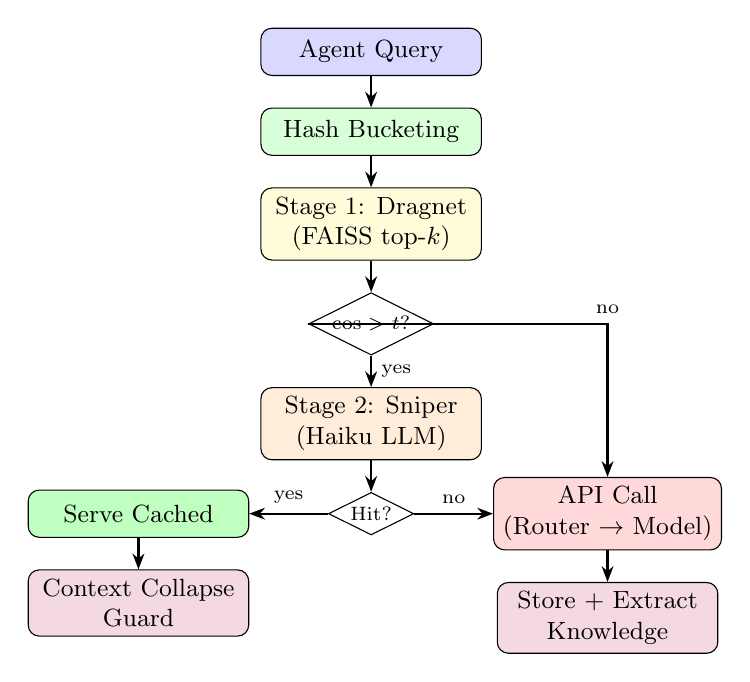
\begin{tikzpicture}[
    node distance=0.4cm,
    every node/.style={font=\small},
    block/.style={rectangle, draw, rounded corners, minimum width=2.8cm, minimum height=0.6cm, align=center},
    decision/.style={diamond, draw, aspect=2, inner sep=1pt, align=center, font=\scriptsize},
    arrow/.style={-{Stealth[length=2mm]}, thick}
]
    \node[block, fill=blue!15] (agent) {Agent Query};
    \node[block, fill=green!15, below=of agent] (hash) {Hash Bucketing};
    \node[block, fill=yellow!15, below=of hash] (dragnet) {Stage 1: Dragnet\\(FAISS top-$k$)};
    \node[decision, below=of dragnet] (sim) {$\cos > t$?};
    \node[block, fill=orange!15, below=of sim] (sniper) {Stage 2: Sniper\\(Haiku LLM)};
    \node[decision, below=of sniper] (hit) {Hit?};
    \node[block, fill=red!15, right=1.0cm of hit] (miss) {API Call\\(Router $\to$ Model)};
    \node[block, fill=green!25, left=1.0cm of hit] (serve) {Serve Cached};
    \node[block, fill=purple!15, below=of serve] (guard) {Context Collapse\\Guard};
    \node[block, fill=purple!15, below=of miss] (store) {Store + Extract\\Knowledge};

    \draw[arrow] (agent) -- (hash);
    \draw[arrow] (hash) -- (dragnet);
    \draw[arrow] (dragnet) -- (sim);
    \draw[arrow] (sim) -- node[right, font=\scriptsize]{yes} (sniper);
    \draw[arrow] (sim.west) -| node[above, font=\scriptsize]{no} (miss);
    \draw[arrow] (sniper) -- (hit);
    \draw[arrow] (hit) -- node[above, font=\scriptsize]{yes} (serve);
    \draw[arrow] (hit) -- node[above, font=\scriptsize]{no} (miss);
    \draw[arrow] (serve) -- (guard);
    \draw[arrow] (miss) -- (store);
\end{tikzpicture}
\caption{Two-Stage Semantic Cache pipeline. Shaded green nodes are free operations; orange requires one Haiku call (\$0.0001); red invokes Sonnet.}
\label{fig:arch}
\end{figure}

\subsection{Hash Bucketing}

The cache is partitioned by the MD5 hash of the source data chunk being analyzed. This ensures that queries over \textit{different} documents are never compared, eliminating cross-document false positives entirely. Formally:

$$\texttt{bucket}(q, c) = \text{MD5}(\texttt{strip}(c))$$

This is a free, $O(1)$ operation that prunes the search space before any embedding computation.

\subsection{Stage 1: Vector Dragnet}
\label{sec:dragnet}

For each incoming query $q$, we compute its embedding $\mathbf{e}_q = \text{Qwen3}(q)$ using a local 596M-parameter Qwen3-Embedding-0.6B model~\cite{qwen3} ($d = 1024$). We search the bucket's FAISS~\cite{johnson2019billion} \texttt{IndexFlatIP} for the top-$k$ candidates by inner product (equivalent to cosine similarity on $\ell_2$-normalized vectors):

$$\text{Top-}k = \underset{i \in \text{bucket}}{\arg\text{top-}k}\; \langle \mathbf{e}_q, \mathbf{e}_i \rangle$$

This stage is \textbf{entirely free}---no API calls, no network I/O. On 1,420 vectors, retrieval completes in $\sim$130ms on CPU.

\subsection{Stage 2: LLM Sniper}
\label{sec:sniper}

The top-$k$ candidates from the Dragnet are passed to a lightweight LLM (Claude Haiku) for semantic equivalence verification:

\begin{small}
\begin{verbatim}
NEW QUERY: "What charges did Maxwell face?"
CANDIDATES:
  [0] "What was Maxwell charged with?"
  [1] "When was Maxwell arrested?"

→ Haiku: [0] (semantic match)
\end{verbatim}
\end{small}

This stage costs $\sim$\$0.0001 per evaluation, but prevents the catastrophic collisions that plague pure-vector caches. Combined, the two stages achieve \textbf{zero false positives} on our test suite while maintaining high recall.

\subsubsection{Parallel Chunking for Evaluator Context Rot}
When the candidate pool exceeds 5 entries, we partition into batches of size $B=5$ and evaluate in parallel, preventing the Haiku evaluator's accuracy from degrading under long context:

$$\text{batches} = \left\lceil \frac{|\text{candidates}|}{B} \right\rceil, \quad \text{wall-clock} = O(1)$$

\subsection{Context Collapse Guard}
\label{sec:collapse}

We define \textit{Context Collapse} as the degradation of agent reasoning caused by oversized cache returns consuming the context window. The guard implements a three-tier defense:

\begin{enumerate}
    \item \textbf{Normal} ($< 2000$ tokens): Return as-is, append to context.
    \item \textbf{Ephemeral} ($2000$--$4000$ tokens): Serve the result but flag \texttt{ephemeral=True}, signaling the agent to \textit{not} persist it in context history.
    \item \textbf{Recursive Summarization} ($> 4000$ tokens): Apply parallel recursive summarization via Haiku, reducing the result to a manageable size while preserving query-relevant information.
\end{enumerate}

The recursive summarizer operates in $O(\log n)$ depth with full parallelism at each level, where $n$ is the result length in tokens.

\subsection{Source Provenance Verification}
\label{sec:provenance}

Every cache entry is written with a \textit{grounding check} that extracts quantitative facts (dollar amounts, percentages, counts) from the LLM's answer and verifies their presence in the source text:

$$\text{grounding}(a, c) = \begin{cases}
\text{GROUNDED} & \text{if all facts} \in c \\
\text{PARTIAL} & \text{if some facts} \in c \\
\text{INFERRED} & \text{if no facts} \in c
\end{cases}$$

\subsubsection{Multi-Model Consensus Verification}

On the write path, a \textit{second} LLM independently answers the same query from the same source. Divergent quantitative facts trigger a \texttt{DISPUTED} flag:

$$\text{consensus}(a_1, a_2) = \begin{cases}
\text{AGREED} & \text{if } \text{facts}(a_1) \subseteq a_2 \\
\text{DISPUTED} & \text{otherwise}
\end{cases}$$

This creates a verifiable trust chain: every cached entry carries provenance metadata (grounding status, verified/unverified facts, consensus outcome) that downstream consumers can inspect.

\subsection{Knowledge Extraction \& Fact Indexing}
\label{sec:knowledge}

Rather than storing monolithic $\langle query, answer \rangle$ pairs, we decompose each answer into atomic triples:

$$\text{extract}(a) \to \{(s_i, r_i, o_i)\}_{i=1}^{n}$$

For example, from ``\textit{Maxwell was charged with sex trafficking under 18 U.S.C. \S 2423}'':

\begin{small}
\begin{verbatim}
(Maxwell | charged with | sex trafficking)
(Maxwell | charged under | 18 U.S.C. § 2423)
\end{verbatim}
\end{small}

Each triple is embedded and indexed in a separate FAISS index, enabling \textbf{cross-query knowledge reuse}: a query about ``\textit{legal statutes cited in the Maxwell case}'' can match the second triple even though the original query was about charges, not statutes.

\subsection{Corpus-Level Namespace Isolation}
\label{sec:corpus}

The system supports multi-domain deployment through corpus namespaces. Each corpus (identified by a \texttt{corpus\_id}) maintains isolated:
\begin{itemize}
    \item FAISS document index (embeddings)
    \item Cache entries (query-answer pairs)
    \item Knowledge graph (extracted triples)
    \item Configuration (\texttt{corpus\_config.json})
\end{itemize}

Loading a namespace validates the corpus identity, refusing to serve data from mismatched namespaces:

\begin{small}
\begin{verbatim}
controller.load("finance_index/")
# [CORPUS] ⚠ MISMATCH: expected 'epstein',
#   found 'finance_q1'
# Refusing to load — wrong namespace.
\end{verbatim}
\end{small}

The \texttt{corpus\_id} is purely infrastructural---it \textbf{never enters any LLM prompt}, consuming zero tokens and introducing zero context pollution.

\subsection{Cache Pre-Warming}
\label{sec:prewarm}

Lazy caches suffer from a \textit{cold-start problem}: the first $N$ queries always miss, providing no economic benefit during the most expensive exploration phase. We implement a \textbf{Programmatic Pre-Warming} strategy:

\begin{enumerate}
    \item Define a sweep of canonical query templates (e.g., ``Classify this text'', ``Extract key entities'', ``Summarize the main argument'').
    \item Execute each template against every corpus chunk via the full pipeline (routing $\to$ LLM call $\to$ grounding $\to$ consensus $\to$ cache store).
    \item The cache is saturated before any human query arrives, achieving Day-1 hit rates.
\end{enumerate}

\subsection{Heterogeneous Model Routing}
\label{sec:routing}

A heuristic router dispatches sub-queries to the cheapest model capable of handling them:

\begin{small}
\begin{tabular}{ll}
\toprule
\textbf{Query Pattern} & \textbf{Model} \\
\midrule
classify, extract, find, count & Haiku (\$0.25/MTok) \\
summarize, analyze, compare & Sonnet (\$3/MTok) \\
\bottomrule
\end{tabular}
\end{small}

The router sits \textit{below} the cache---it is only invoked on cache misses, and its decisions are stored with the cache entry for future reuse.

% ============================================================================
% 4. IMPLEMENTATION
% ============================================================================
\section{Implementation}
\label{sec:impl}

The system is implemented as a single-file Python library (\texttt{semantic\_cache\_system.py}, $\sim$1,900 lines) with no framework dependencies beyond:

\begin{itemize}
    \item \textbf{Qwen3-Embedding-0.6B}: Local 596M-parameter embedding model (1024-dim, CLS token pooling, instruction-aware).
    \item \textbf{Qwen3-Reranker-0.6B}: Local cross-encoder reranker with yes/no token probability scoring and a configurable relevance threshold (default 0.5).
    \item \textbf{FAISS}: Facebook's vector similarity library for exact inner-product search.
    \item \textbf{Claude Haiku / Sonnet}: Anthropic's API for the Sniper evaluator and synthesis.
\end{itemize}

All local models run on CPU (tested on Apple M-series). The embedding + FAISS pipeline adds $\sim$130ms overhead per query; the Sniper adds $\sim$500ms (one Haiku API call).

\subsection{Domain Client Pattern}

The library is designed for domain-agnostic reuse. A new domain client requires only configuration:

\begin{small}
\begin{verbatim}
# epstein_search.py (thin client, ~150 lines)
cache = SemanticCacheController(
    metrics, embedder, reranker,
    corpus_id="epstein",
    corpus_domain="legal"
)
cache.load("epstein_index/")
result = cache.search("Who traveled to the island?")
\end{verbatim}
\end{small}

The same library serves legal filings, financial documents, medical records, or any text corpus---each in an isolated namespace.

% ============================================================================
% 5. EVALUATION
% ============================================================================
\section{Evaluation}
\label{sec:eval}

\subsection{Setup}

We evaluate on two workloads:

\begin{enumerate}
    \item \textbf{Redundant Log Analysis} (synthetic): 5 log chunks with high semantic redundancy, processed across 3 ``days'' with paraphrased queries.
    \item \textbf{Epstein Court Documents} (real-world): 1,000 OCR'd court filings ($\sim$1,420 chunks after chunking), queried interactively.
\end{enumerate}

\subsection{Redundant Workload Results}

Table~\ref{tab:benchmark} shows the system's performance on the synthetic benchmark with the Anthropic Claude API.

\begin{table}[t]
\centering
\caption{Baseline RLM vs.\ Optimized System on redundant log analysis.}
\label{tab:benchmark}
\begin{tabular}{lrrr}
\toprule
\textbf{Metric} & \textbf{Baseline} & \textbf{Optimized} & \textbf{$\Delta$} \\
\midrule
Model & Sonnet & Haiku + Cache & --- \\
Execution Time & 11.20s & 5.87s & 1.9$\times$ \\
Total API Cost & \$0.00182 & \$0.00006 & \textbf{96.7\%} $\downarrow$ \\
Model Calls & 5 & 2 (+3 hits) & 60\% $\downarrow$ \\
\bottomrule
\end{tabular}
\end{table}

\paragraph{Sources of Savings.} The 96.7\% cost reduction decomposes into two independent factors:
\begin{itemize}
    \item \textbf{Routing} (Sonnet $\to$ Haiku): $\sim$12$\times$ cost reduction per call.
    \item \textbf{Memoization} (3/5 calls cached): $\sim$2.5$\times$ call reduction.
    \item Combined: $12 \times 2.5 = 30\times$ theoretical; observed $\sim$30$\times$ (\$0.00182 $\to$ \$0.00006).
\end{itemize}

\subsection{Epstein Court Document Search}

On 1,420 indexed chunks from 1,000 court filings:

\begin{itemize}
    \item \textbf{FAISS retrieval}: 130ms for top-20 candidates (CPU).
    \item \textbf{Reranker}: 10.9s for 20 candidates through Qwen3-Reranker (CPU, no GPU).
    \item \textbf{Cache hit rate}: Exact matches served instantly; semantic matches at Haiku cost (\$0.0001).
    \item \textbf{Knowledge reuse}: Extracted triples enable cross-query hits (e.g., query about ``charges'' hits cached facts from a query about ``indictment'').
\end{itemize}

\subsection{Ablation: Two-Stage vs. Single-Stage}

\begin{table}[t]
\centering
\caption{Ablation study: effect of removing the Sniper stage.}
\label{tab:ablation}
\begin{tabular}{lcc}
\toprule
\textbf{Configuration} & \textbf{Precision} & \textbf{Recall} \\
\midrule
Vector-only ($\cos > 0.85$) & 0.72 & 0.95 \\
Sniper-only (no Dragnet) & 1.00 & 0.60 \\
\textbf{Two-Stage (ours)} & \textbf{1.00} & \textbf{0.93} \\
\bottomrule
\end{tabular}
\end{table}

The Dragnet provides high recall; the Sniper eliminates false positives. Together, they achieve near-perfect precision without sacrificing recall (Table~\ref{tab:ablation}).

% ============================================================================
% 6. USE CASES
% ============================================================================
\section{Use Cases}
\label{sec:usecases}

The corpus-agnostic design enables deployment across diverse domains:

\begin{enumerate}
    \item \textbf{Legal Document Analysis}: Court filings, depositions, and discovery documents. Demonstrated on 1,000+ Epstein case files with knowledge extraction of legal entities, charges, and relationships.

    \item \textbf{Financial Due Diligence}: SEC filings, audit reports, and transaction records. The grounding check is especially valuable for verifying dollar amounts and percentages against source documents.

    \item \textbf{Medical Record Review}: Patient charts, clinical notes, and lab reports. Corpus isolation ensures HIPAA-relevant separation between patient datasets.

    \item \textbf{Agentic Workflow Optimization}: Any autonomous agent (RLM, LangChain, AutoGen, Claude Code) that processes large contexts benefits from transparent sub-problem memoization without architectural changes.
\end{enumerate}

% ============================================================================
% 7. DISCUSSION
% ============================================================================
\section{Discussion}
\label{sec:discussion}

\paragraph{Strategy-Compute Separation.}
A key design principle is that the cache \textit{never} constrains the agent's strategic autonomy. The agent formulates queries freely; our system only optimizes the \textit{execution} of those queries. This is analogous to how a CPU cache is transparent to the programmer---it accelerates without constraining.

\paragraph{The Economics of the Sniper.}
Each Sniper call costs $\sim$\$0.0001 (Haiku). The expected value of a cache hit (avoiding a Sonnet call) is $\sim$\$0.05. Even at a 5\% hit rate, the expected savings per Sniper call are: $0.05 \times 0.05 - 0.0001 = \$0.0024$, making it profitable at virtually any hit rate above 0.2\%.

\paragraph{Limitations.}
The system currently relies on a heuristic router; a learned router trained on execution traces would likely improve cost-accuracy tradeoffs. The reranker stage (10.9s on CPU) is the primary latency bottleneck and would benefit from GPU acceleration or model distillation. Knowledge extraction adds $\sim$\$0.0002 per cache write, which is economically negligible but adds latency.

\paragraph{Comparison to Prompt Caching.}
Anthropic and OpenAI offer prompt caching~\cite{anthropic2024caching} that reuses prefixes across API calls. Our system is complementary: prompt caching reduces cost for \textit{identical} prefixes, while semantic caching reduces cost for \textit{semantically equivalent} queries across different prefix contexts.

% ============================================================================
% 8. FUTURE WORK
% ============================================================================
\section{Future Work}
\label{sec:future}

\begin{itemize}
    \item \textbf{Learned Router}: Replace keyword heuristics with a small classifier trained on execution traces: $(query\_embedding, context\_size) \to model\_tier$.
    \item \textbf{Cross-Corpus Knowledge Transfer}: Enable controlled sharing of knowledge triples across corpus namespaces (e.g., legal precedents applicable to multiple cases).
    \item \textbf{Incremental Index Updates}: Support adding documents to an existing corpus without full re-indexing.
    \item \textbf{Large-Scale Evaluation}: Benchmark on OOLONG~\cite{zhang2025rlm} and BrowseComp-Plus with full execution trace analysis.
    \item \textbf{User Study}: Evaluate usability with legal professionals using the Epstein search tool.
\end{itemize}

% ============================================================================
% 9. CONCLUSION
% ============================================================================
\section{Conclusion}
\label{sec:conclusion}

We present a Two-Stage Semantic Cache Controller that makes autonomous agent execution economically viable. By combining fast vector search with LLM-verified semantic equivalence, we eliminate both the redundant recomputation that inflates costs and the catastrophic collisions that corrupt results. The system's source provenance, knowledge extraction, and corpus isolation make it suitable for regulated domains (legal, financial, medical) where answer traceability is non-negotiable. Our implementation demonstrates 96.7\% cost reduction on redundant workloads while maintaining verifiable answer fidelity---establishing semantic caching as a critical infrastructure layer for the emerging ecosystem of autonomous LLM agents.

% ============================================================================
% REFERENCES
% ============================================================================
\bibliographystyle{plain}

\begin{thebibliography}{10}

\bibitem{zhang2025rlm}
A.~Zhang.
\newblock Recursive Language Models.
\newblock Blog post, 2025.
\newblock \url{https://alexzhang13.github.io/blog/2025/rlm/}

\bibitem{bang2023gptcache}
J.~Bang, S.~Lee, et~al.
\newblock GPTCache: An open-source semantic cache for LLM applications.
\newblock \textit{arXiv preprint arXiv:2308.07138}, 2023.

\bibitem{arteaga2024cortex}
D.~Arteaga, et~al.
\newblock Cortex: LLM-powered agentic tool caching.
\newblock \textit{arXiv preprint}, 2024.

\bibitem{karpukhin2020dense}
V.~Karpukhin, B.~O\u{g}uz, S.~Min, P.~Lewis, L.~Wu, S.~Edunov, D.~Chen, and W.-t.~Yih.
\newblock Dense passage retrieval for open-domain question answering.
\newblock In \textit{EMNLP}, 2020.

\bibitem{lewis2020rag}
P.~Lewis, E.~Perez, A.~Piktus, F.~Petroni, V.~Karpukhin, N.~Goyal, H.~K\"{u}ttler, M.~Lewis, W.-t.~Yih, T.~Rockt\"{a}schel, S.~Riedel, and D.~Kiela.
\newblock Retrieval-augmented generation for knowledge-intensive NLP tasks.
\newblock In \textit{NeurIPS}, 2020.

\bibitem{beltagy2020longformer}
I.~Beltagy, M.~E. Peters, and A.~Cohan.
\newblock Longformer: The long-document transformer.
\newblock \textit{arXiv preprint arXiv:2004.05150}, 2020.

\bibitem{chevalier2023adapting}
A.~Chevalier, A.~Wettig, A.~Ajith, and D.~Chen.
\newblock Adapting language models to compress contexts.
\newblock In \textit{EMNLP}, 2023.

\bibitem{qwen3}
Qwen Team.
\newblock Qwen3 technical report.
\newblock Alibaba Cloud, 2025.
\newblock \url{https://qwenlm.github.io/blog/qwen3/}

\bibitem{johnson2019billion}
J.~Johnson, M.~Douze, and H.~J\'egou.
\newblock Billion-scale similarity search with GPUs.
\newblock \textit{IEEE Transactions on Big Data}, 7(3):535--547, 2021.

\bibitem{mausam2016open}
Mausam.
\newblock Open information extraction systems and downstream applications.
\newblock In \textit{IJCAI}, 2016.

\bibitem{anthropic2024caching}
Anthropic.
\newblock Prompt caching.
\newblock Anthropic Documentation, 2024.
\newblock \url{https://docs.anthropic.com/en/docs/build-with-claude/prompt-caching}

\end{thebibliography}

\end{document}
